
\section{Background}
\label{basicModel}

\subsection{Pitman-Yor Process}

The Pitman-Yor process is a generalization of the Dirichlet process with three parameters.   If $\G \sim \PY(d,c,\G_0)$ we say $\G$ is distributed according to a Pitman-Yor process with discount parameter $d$, concentration parameter $c$, and base measure $\G_0$. In the case that $d = 0$ the Pitman-Yor process reduces to the Dirichlet process \cite{Pitman1997}.  A simple model using the Pitman-Yor process, where a distribution is drawn from a Pitman-Yor process and then samples are drawn from the resulting distribution, can be written as follows:

\begin{eqnarray*}
\G | d,c,\G_0 &\sim& \PY(d,c,\G_0)\\
\theta_i | \G &\sim& \G  \hspace{.5cm} i = 1, \dots, N
\end{eqnarray*}

It is possible to work in a representation where the random distribution $\G$ is analytically marginalized out.  One way to draw a sample $\{ \theta_j \}_{j = 1}^N$ in this representation is to use a two step process.  The first step produces a partition of the integer $N$ which follows the two parameter Ewen's sampling distribution ($\ES_N(d,c)$) \cite{Ewens1995}.  The second step assigns to each of the $K$ segments of the partition a parameter $\psi_k$ drawn independently from $\G_0$.  We set $\theta_j = \psi_k$ for all integers $j$ in segment $k$ of the partion \cite{Blackwell1973}.

Samples can be drawn from the Ewen's sampling distribution using the Chinese Restaurant Process (CRP).  Since the connection between the CRP and the Ewen's sampling distribution is essential to developments later in the paper we describe here the CRP in detail. We imagine a restaurant with an infinite number of tables, capable of holding an infinite number of customers.  The first customer in the CRP sits down at an empty table.  Customers $2 \dots N$ are seated sequentially by seating the $j^{\mathrm{th}}$ customer at a table drawn from the following distribution:

\begin{eqnarray*}
p(\textrm{occupied table}\; i |\textrm{ previous}) &=& \frac{n_i - d}{j-1+ c}\\
p(\textrm{unoccupied table} | \textrm{ previous}) &=& \frac{t_{j-1}d +c}{j-1+c}
\end{eqnarray*}

where $n_i$ is the number of customers already sitting at table $i$, $t_{j-1}$ is the number of tables occupied by the first $j-1$ customers, and previous refers to the seating arrangement of the first $j-1$ customers.  The final seating arrangement in the restaurant defines a partition of the integer $N$ which follows the $\ES_N(d,c)$ distribution \cite{Pitman1995}.  To complete the process of generating a sample $\{ \theta_j \}_{j = 1}^N$ we must endow each occupied table in the restaurant with a parameter $\psi_k$ drawn independently from $\G_0$.  We set $\theta_j = \psi_k$ if customer $j$ is sitting at table $k$.


\subsection{Hierarchical Pitman-Yor Process}

%Recent research has produced a spate of new hierarchical models using the Pitman-Yor process \cite{Teh2006b} \cite{Teh2006a}.  
An an example hierarchical Pitman-Yor process is 

\begin{eqnarray*}
\G_1|d_1, c_1, \G_0 &\sim& \PY(c_1,c_1,\G_0)\\
\G_2 | d_2, c_2, \G_1 &\sim& \PY(d_2,c_2, \G_1)\\
\theta_i | \G_2 &\sim& \G_2 \hspace{.5cm} i = 1,\dots, N.
\end{eqnarray*}

To obtain a sample from the hierarchical Pitman-Yor process it is again possible to work in a representation where $G_2$ and $G_1$ are analytically marginalized out. One can generate samples in this representation by recursively applying the algorithm for the single Pitman-Yor process.  To draw a sample $\{ \theta_j \}_{j = 1}^N$ we again need to produce a partition of the integer $N$ following the $\ES_N(d_2,c_2)$ distribution.  This can be achieved using the CRP.  In Figure~\ref{figHPY} this is represented by the restaurant corresponding to $\G_2$. We will denote the number of tables in the child restaurant as $K_2$.  Each of the $K_2$ tables must be endowed with a parameter $ \psi_{2k}$ drawn independently from $\G_1$.  Since $\G_1$ has been marginalized out we obtain $\{ \psi_{2k} \}_ {k = 1}^{K_2}$ by again using the procedure for the single Pitman-Yor process.  A partition following the $\ES_{K_2}(d_1,c_1)$ distribution is produced via the CRP.  This is represented in Figure~\ref{figHPY} by the restaurant corresponding to $\G_1$. We denote the number of tables in the parent restaurant as $K_1$.   Each of the $K_1$ tables must be endowed with a parameter $\{ \psi_{1k} \}_{ k = 1}^{K_1}$ drawn independently from $\G_0$.  We set $\psi_{2k}  = \psi_{1m}$ if in the parent restaurant customer $k$ is sitting at table $m$ and we set $\theta_j = \psi_{2k}$ if in the child restaurant customer $j$ is sitting at table $k$.

\begin{figure}[t] 
	\begin{center}
		\label{figHPY}
		\scalebox{.25}{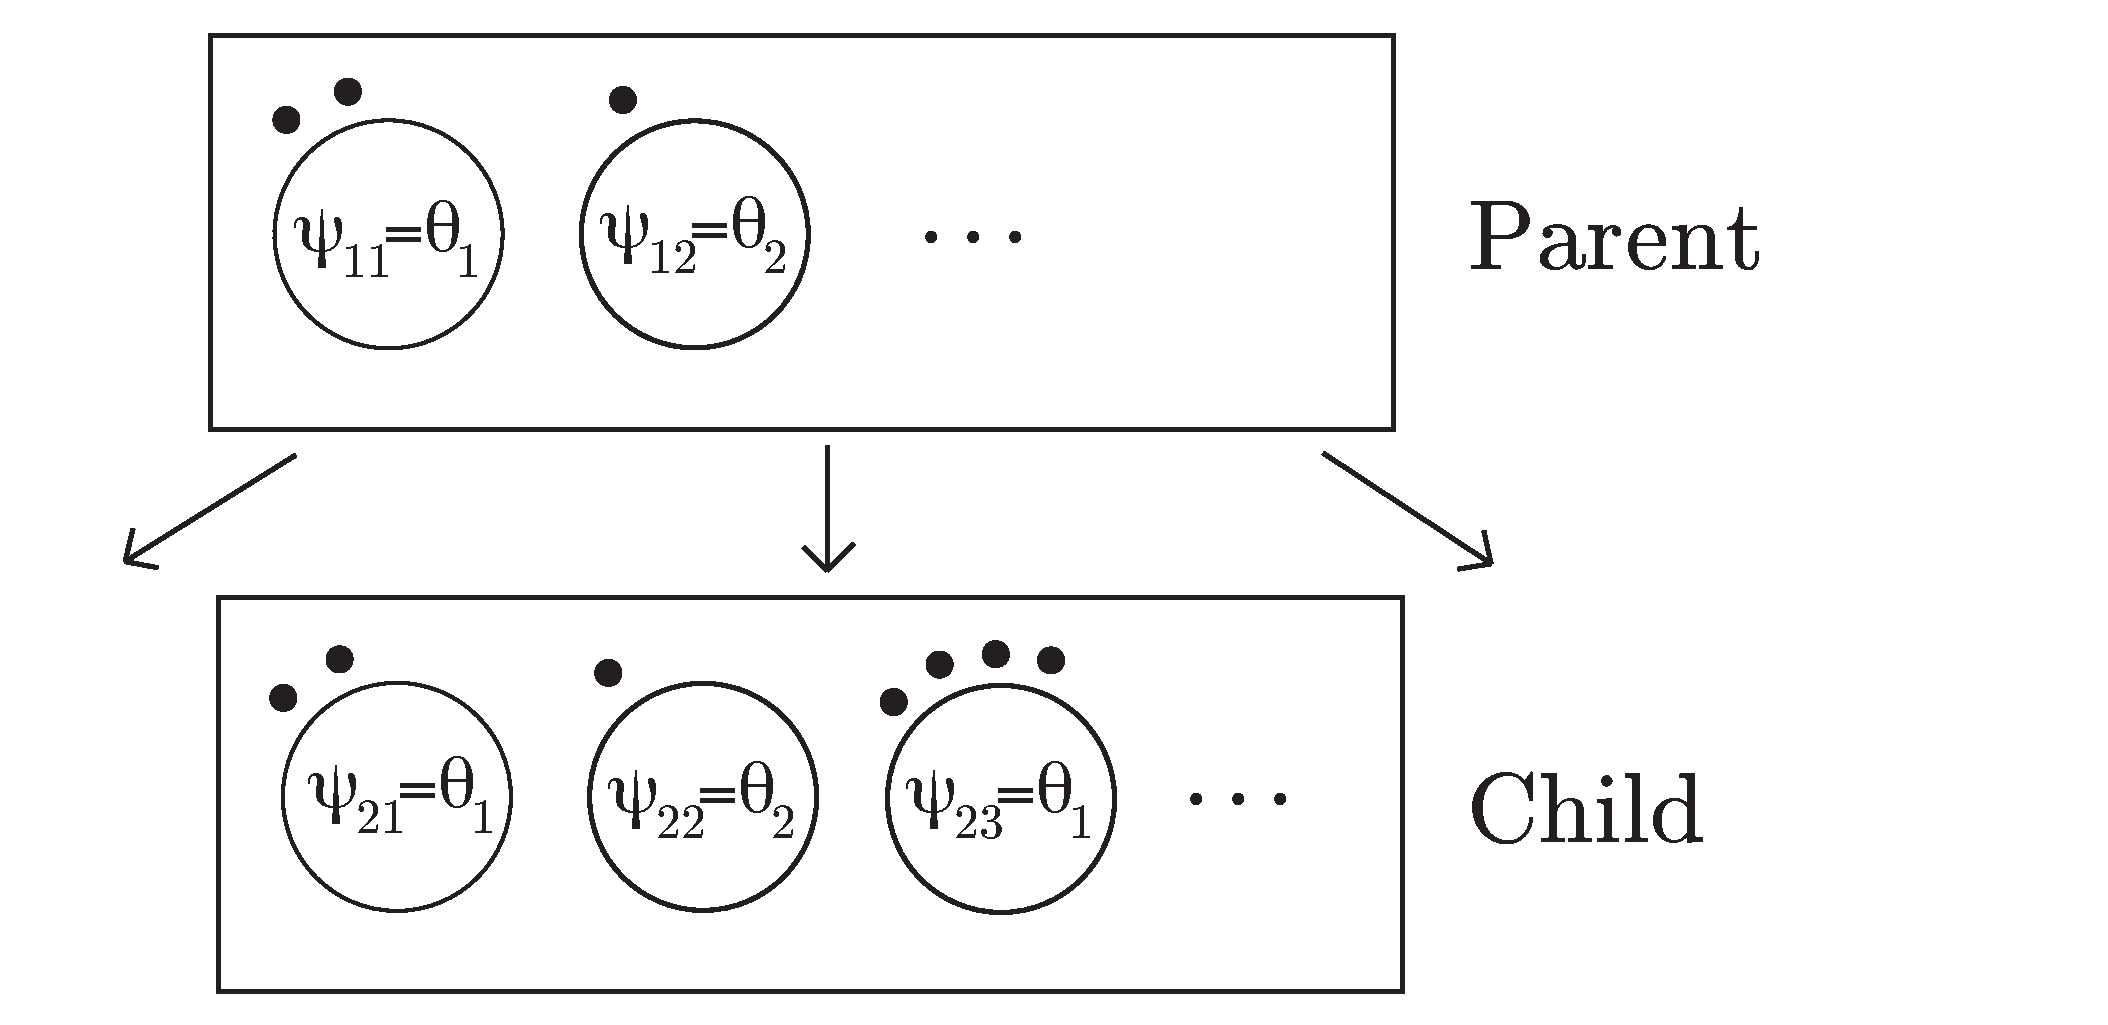
\includegraphics{figure1.pdf}} % [clip=true, viewport= 1in 1in 9in 9in]
		\caption{Final state of an example CRF process.}
	\end{center} 

\end{figure} 

\comment{An example is shown in Figure~\ref{figHPY} in which the CRP process for the child restaurant resulted in three tables ($K_2 = 3$).  Therefore, three parameters must have been drawn from $\G_1$.  Since $\G_1$ is marginalized out we again revert to the procedure for a single Pitman-Yor process. The CRP for the parent restaurant resulted in two tables ($K_1 = 2$).  $\psi_{11}$ and $\psi_{12}$ are drawn independently from the base distribution $\G_0$.  $\{ \psi_{2k} \}_{k = 1}^{K_1}$ is equal to $\{ \psi_{11}, \psi_{11}, \psi_{12} \}$ and finally  $\{ \theta_j \}_{j = 1}^7 = \{ \psi_{11}, \psi_{11}, \psi_{12},\psi_{11},\psi_{11}, \psi_{11}, \psi_{11}\}$.}

The recursive application of the CRP in a hierarchical model is known as the Chinese restaurant franchise (CRF) \cite{Teh2006b}.  The number of child restaurants is not restricted to one, as indicated by the dashed lines in Figure~\ref{figHPY}.  Furthermore, the recursive nature of the CRF makes extensions to deeper hierarchies straightforward. For more more detail refer to \cite{Teh2006b, Teh2006a}.

\subsection{Sequence Memoizer}

The sequence memoizer (SM) \cite{Wood2009} is a model for discrete sequence data based on an unbounded depth hierarchical Pitman-Yor process. We can write the model as:

\begin{eqnarray*}
	\G_{[]} | \mathcal{U}_{\Sigma}, d_0 &\sim& \PY(d_0, 0, \mathcal{U}_{\Sigma }) \\
	\G_{\bf{u}} | \G_{\sigma(\bf{u})}, d_{|\bf{u}|} &\sim& \PY(d_{|\bf{u}|}, 0, \G_{\sigma(\bf{u})}) \hspace{.35cm} \forall \bf{u} \in \Sigma^+\\
	\theta_n | \theta_{n-1}  \ldots \theta_1 = \bf{u} &\sim& \G_{\bf{u}}
\end{eqnarray*}

where $\mathcal{U}_{\Sigma }$ is a uniform distribution over the set of symbols, $\bf{u}$ is a particular context, $\Sigma^+$ is the set of all such contexts, and $\sigma(\bf{u})$ is the context $\bf{u}$ modified by removing the most distant symbol.  We assume $| \Sigma | < \infty$. 

\begin{figure}[t] 
	\label{figprefixtree}
	\begin{center}
		\scalebox{.5}{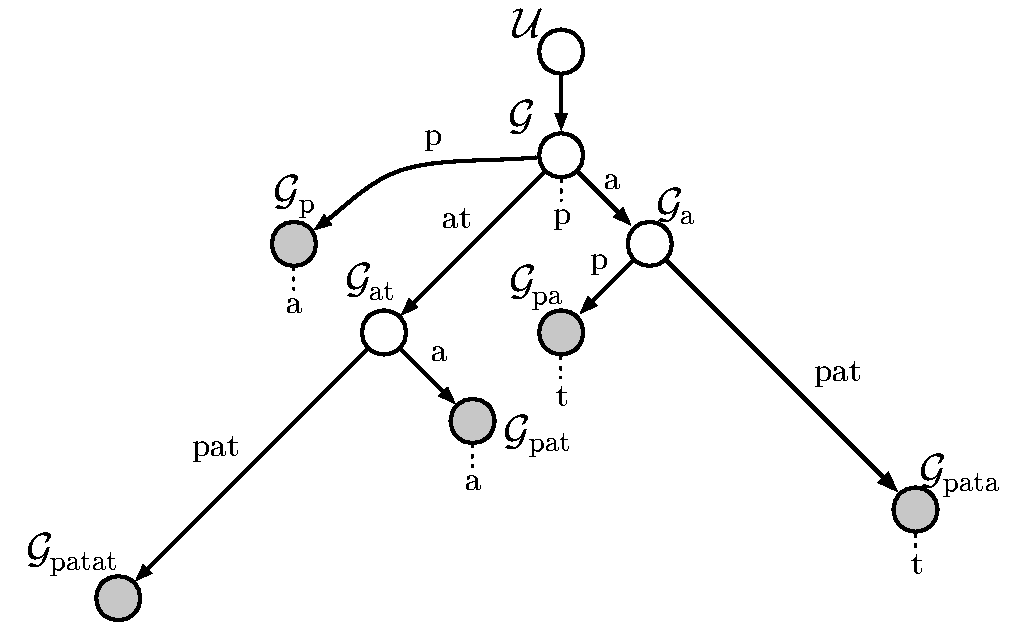
\includegraphics{prefix_tree.pdf}} % [clip=true, viewport= 1in 1in 9in 9in]
		\caption{An example prefix tree for the sequence $patat$}.
	\end{center} 
\end{figure} 

Figure~\ref{figprefixtree} shows the graphical model instantiated by the sequence $patat$.  Note that in the SM graphical model, nodes that are not branching nodes and are not associated with observed data are not instantiated.  This is because of a result from \cite{Pitman1999,Ho2006} showing that two Pitman-Yor processes can be analytically integrated against one another.  Note that this result is different than the result from \cite{Blackwell1973} allowing for the representation we are using which analytically integrates out each random distribution separately\comment{whiskey tango foxtrot?}.  The node labeled $\G_{patat}$ is only shown in the graphical model to indicate that the next symbol in the sequence will come from this distribution.

Inference in the SM model is performed in the Chinese restaurant franchise respresentation. Inference takes worst case $\mathcal{O}(n^2)$ time and requires $\mathcal{O}(n)$ space where $n$ is the length of the sequence. Quadratic time stems from the fact that seating a customer in the appropriate restaurant may require seating a customer in all of the restaurants above it.  The length of this path is bounded by the length of the sequence. Each restaurant requires constant space because a restaurant need only maintain a constant number of summary statistics, the total number of customers and the total number of tables present of each type.\footnote{For symbol sets of finite cardinality.} Note this representation requires reinstantiation of the full restaurant state for some steps of inference which can be done by exploiting exchangeability.  The fact that a restaurant can be represented allows the full model to be represented in $\mathcal{O}(n)$ space.

In most applications $\mathcal{O}(n)$ space is acceptable, but for sequence modeling of extremely long sequences it is problematic.  Tasks such as compression often encounter sequences which make the SM an impractical option.  